\documentclass[crop,tikz,border=1px]{standalone}

\usetikzlibrary{arrows,positioning,scopes,automata,calc}

\begin{document}
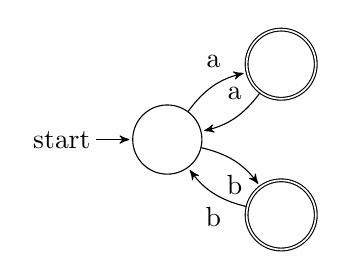
\begin{tikzpicture}[->,>=stealth',shorten >=1pt,auto,
  inner sep=2pt,minimum size=.6cm,
  mystate/.style={state,text centered}]

  \node[accepting,mystate] (q1)  {};
  \node[accepting,mystate] (q2) [below=of q1] {};
  \coordinate (mid) at ($(q1)!0.5!(q2)$);
  \node[initial,mystate] (q0) [left=of mid] {};

  {[every edge/.append style={bend left=20}]
    \path (q0) edge node [above] {a} (q1)
          (q1) edge node [above] {a} (q0)

          (q0) edge node [below] {b} (q2)
          (q2) edge node [below] {b} (q0);
  }

\end{tikzpicture}
\end{document}
